\documentclass[11pt,a4paper]{article}
\let\originalpercent\%
\usepackage[spanish,es-nodecimaldot]{babel}
\AtBeginDocument{\let\%\originalpercent}
\usepackage[margin=23mm]{geometry}
\usepackage{microtype,amsmath,amssymb,graphicx,booktabs,longtable,tabularx,array,xcolor,float,fancyhdr,enumitem}
\usepackage[colorlinks=true,linkcolor=black,urlcolor=blue!55!black,citecolor=blue!55!black]{hyperref}
\graphicspath{{../../img/}}
% Identidad: Manual resumido de marca CUC, edición publicada en agosto de 2024.
% Logo vectorial oficial, sin reconstrucción ni modificación de sus elementos.
\usepackage{fontspec}
\usepackage{unicode-math}
\setmathfont{Latin Modern Math}
\defaultfontfeatures{Ligatures=TeX}
\setmainfont{RedHatDisplay}[Path=fuentes/,Extension=.ttf,UprightFont=*-Regular,BoldFont=*-Bold,ItalicFont=*-Italic]
\setsansfont{RedHatDisplay}[Path=fuentes/,Extension=.ttf,UprightFont=*-Regular,BoldFont=*-Bold,ItalicFont=*-Italic]
\definecolor{cucrojo}{HTML}{A3161A}
\definecolor{cucoro}{HTML}{C9A227}
\definecolor{cucgris}{HTML}{595959}
\definecolor{cucplata}{HTML}{CCCCCC}
\newcommand{\logocuc}[1]{
\includegraphics[width=#1]{marca/cuc-logo-vector.pdf}}

\usepackage{titlesec}
\titleformat{\section}{\Large\bfseries\color{cucrojo}}{\thesection.}{.65em}{}
\titleformat{\subsection}{\large\bfseries}{\thesubsection.}{.65em}{}
\hypersetup{linkcolor=cucrojo,urlcolor=cucrojo,citecolor=cucrojo}
\setlength{\headheight}{30pt}
\renewcommand{\headrule}{\hbox to\headwidth{\color{cucrojo}\leaders\hrule height .5pt\hfill}}
\definecolor{azul}{HTML}{164E63}
\setlength{\parindent}{0pt}\setlength{\parskip}{6pt}
\setlist{nosep,leftmargin=*}
\pagestyle{fancy}\fancyhf{}\fancyhead[L]{\logocuc{32mm}}\fancyhead[R]{\small Electrónica II · Ecualizador ESP32}\fancyfoot[C]{\thepage}
\newcommand{\figura}[3][.9]{\begin{figure}[H]\centering\includegraphics[width=#1\linewidth,height=.34\textheight,keepaspectratio]{#2}\caption{#3}\end{figure}}
\title{\textbf{Ecualizador de audio de tres bandas\\con analizador de espectro en ESP32}}
\author{Leo Rojas \and David Orozco \and Manuel Castilla}
\date{Universidad de la Costa · Ingeniería Electrónica\\Electrónica II · Fase 2 del proyecto de aula\\22 de octubre de 2026}
\begin{document}
\hypersetup{pageanchor=false}
\begin{titlepage}
\centering
\vspace*{5mm}
\logocuc{105mm}\par
\vspace{16mm}
{\color{cucrojo}\rule{\linewidth}{1.2pt}}\par
\vspace{6mm}
{\small\bfseries ELECTRÓNICA II / PROYECTO DE AULA / FASE 2}\par
\vspace{7mm}
{\Huge\bfseries Ecualizador de audio\par de tres bandas}\par
\vspace{4mm}
{\Large Analizador de espectro en ESP32}\par
\vspace{6mm}
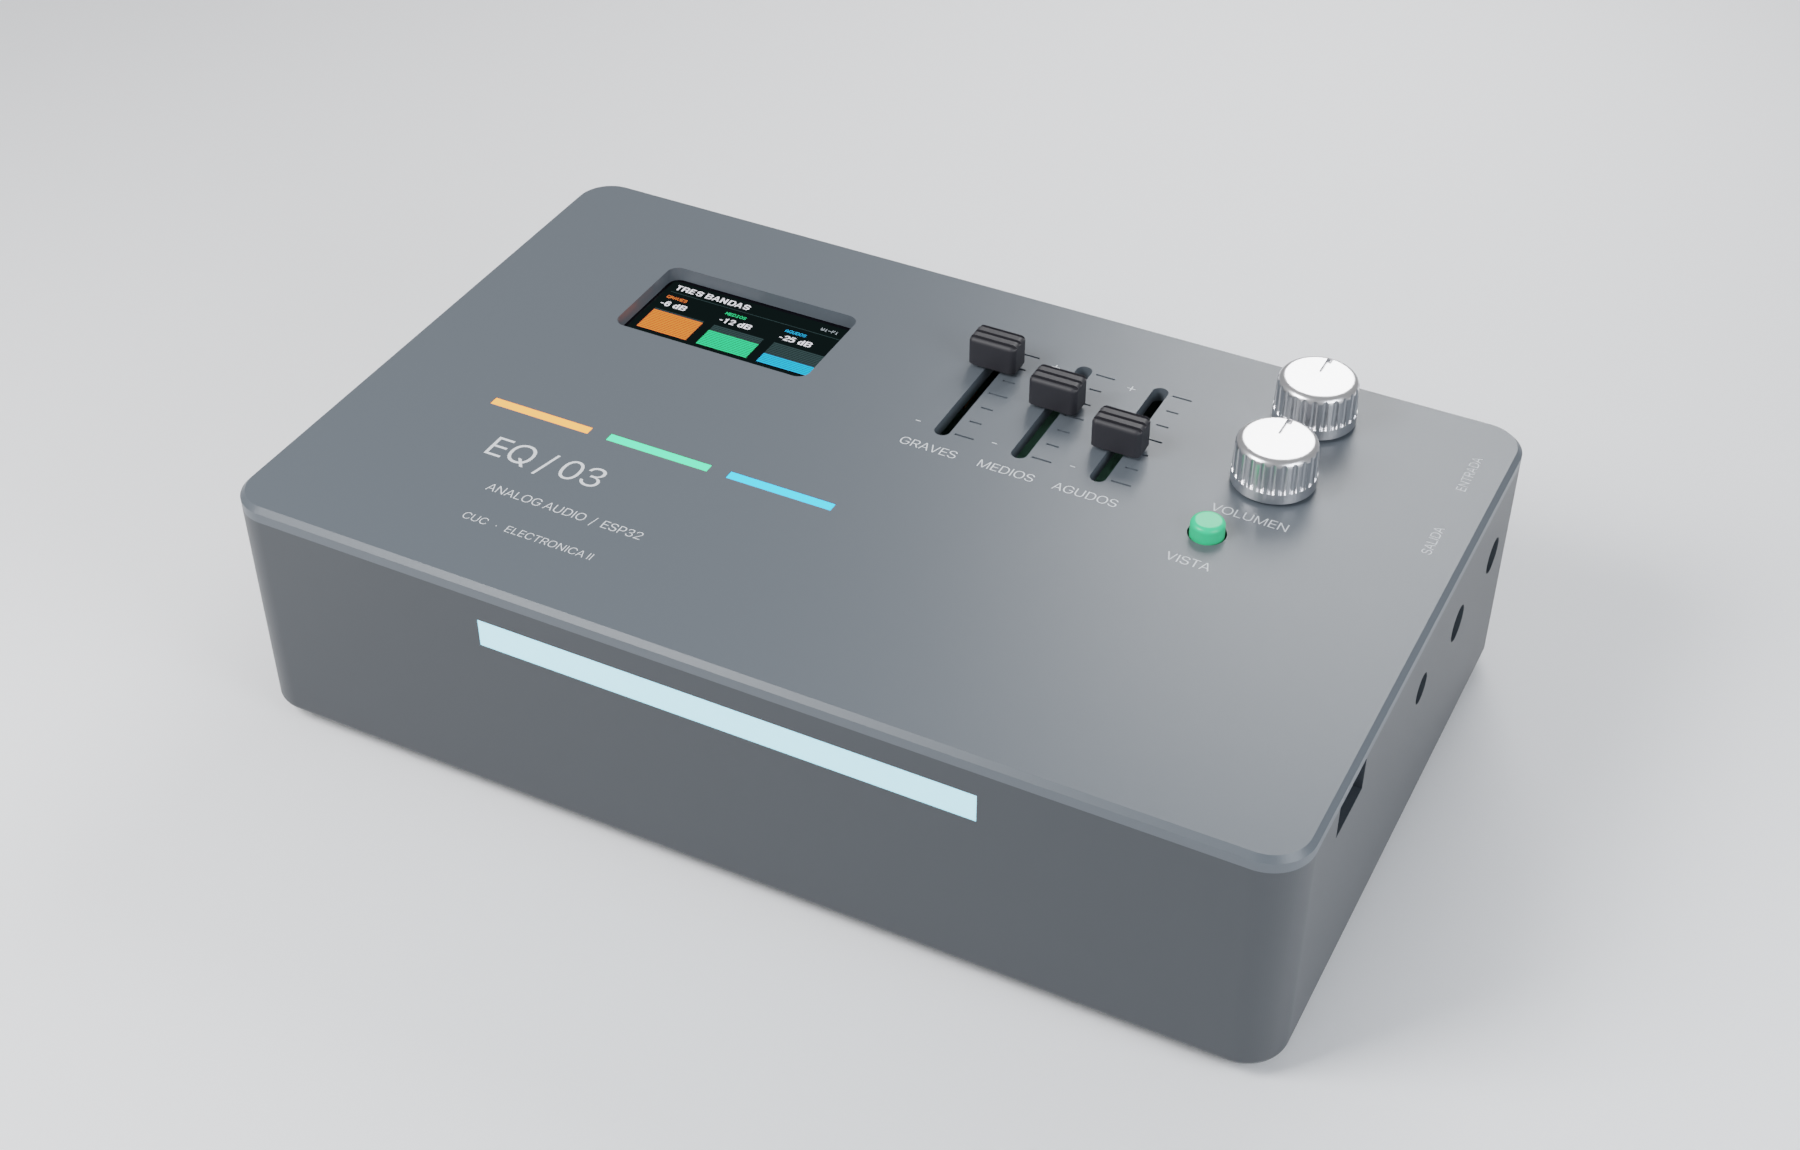
\includegraphics[width=.9\linewidth,height=78mm,keepaspectratio]{3d-gabinete-cerrado.png}\par
{\footnotesize Diseño del gabinete con pantalla Waveshare y canales NeoPixel. Render CAD.}\par
\vfill
{\large Leo Rojas · David Orozco · Manuel Castilla}\par
\vspace{5mm}
Ingeniería Electrónica · Universidad de la Costa\par
Barranquilla · 22 de octubre de 2026\par
\vspace{5mm}
{\color{cucrojo}\rule{\linewidth}{1.2pt}}
\end{titlepage}
\hypersetup{pageanchor=true}
\textbf{Alcance de esta entrega.} Se presentan el diseño, las simulaciones, la PCB, el gabinete y el firmware. Los resultados numéricos corresponden a simulaciones y pruebas en computador.
\tableofcontents\newpage
\section{Introducción y elección de la propuesta}
El ecualizador permite ajustar graves, medios y agudos de una señal de línea. La cadena analógica tiene puntos de medida entre etapas para comparar su respuesta con los cálculos y las simulaciones. El audio de línea se mezcla a mono, se acondiciona alrededor de una referencia de tensión, se separa con filtros activos y se vuelve a sumar después de ajustar cada banda.

El ESP32 se utiliza para observar esa cadena: lee tres detectores de pico y calcula el espectro de la salida. La ecualización ocurre en los amplificadores operacionales; la pantalla y el enlace Wi-Fi muestran las medidas. Esto permite comparar el sonido, las señales del osciloscopio y la respuesta calculada.

En la Fase 1 se plantearon un preamplificador con analizador, un ecualizador de tres bandas y un monitor de ECG. Se escogió el ecualizador porque permite trabajar con realimentación, filtros, suma de señales y detección de picos en un mismo circuito. Se incorporó el análisis espectral de la primera propuesta. El documento original se conserva en \texttt{docs/fase1/Propuestas\_Electronica\_II.pdf}.

La pantalla es una Waveshare de 1,9 pulgadas, 170 × 320 píxeles y controlador ST7789V2. Dos tramos de tira NeoPixel iluminan el interior de la caja y reciben alimentación de 5 V.

\section{Objetivos}
\subsection{Objetivo general}
Desarrollar un ecualizador de audio de tres bandas que permita ajustar graves, medios y agudos, reproducir la señal procesada y visualizar sus niveles y espectro mediante un ESP32.
\subsection{Objetivos específicos}
\begin{enumerate}
\item Diseñar los filtros activos y las etapas de ajuste y suma para controlar las tres bandas de audio.
\item Integrar la salida de línea, el amplificador y los controles en un equipo con PCB de una cara y gabinete propio.
\item Programar la adquisición y visualización con el ESP32, y evaluar el equipo mediante simulación y mediciones de laboratorio.
\end{enumerate}

\section{Estado del arte}
Los filtros Sallen-Key, el procesamiento digital con ADAU1701 y WLED Audio Reactive ofrecen referencias para el filtrado y la visualización. En este proyecto se conservan los filtros analógicos para medir sus nodos en el laboratorio.
\begin{table}[H]\small\centering
\begin{tabularx}{\linewidth}{p{30mm}XX}\toprule
Antecedente & Qué aporta & Relación con el proyecto\\\midrule
Filtros Sallen-Key \cite{karki} & Implementación activa con un operacional por sección de segundo orden. & Sus relaciones entre $R$, $C$, frecuencia y amortiguamiento sirven para dimensionar las bandas.\\
ADAU1701 y SigmaStudio \cite{adau} & Procesamiento digital programable; incorpora dos ADC y cuatro DAC. & Es una alternativa para ecualización flexible. Aquí se conservan filtros analógicos para medir sus nodos.\\
WLED Audio Reactive \cite{wled} & Análisis de audio para efectos LED; admite micrófonos y distintas opciones de entrada de línea. & Es una referencia de visualización con ESP32. La iluminación de esta entrega es fija y tenue; no se presenta como un analizador adicional.\\\bottomrule
\end{tabularx}\caption{Comparación basada en documentación de los fabricantes y del proyecto WLED.}
\end{table}
La decisión de diseño es mantener separadas la ruta de audio y la ruta de observación. Una falla del enlace Wi-Fi no necesita interrumpir el filtrado analógico. A cambio, la precisión del análisis queda limitada por el ADC interno, el filtro previo y la temporización del muestreo.

\section{Marco teórico y cálculos}
\subsection{Alimentación única y referencia de señal}
\figura[.9]{circuitos/referencia.pdf}{Alimentación analógica y referencia VREF con U1A.}
La señal de audio cambia de polaridad, mientras que los MCP6004 trabajan entre GND y la alimentación analógica. Las unidades U1E–U4E muestran los pines de alimentación de los MCP6004: pin 4 a la alimentación y pin 11 a GND. C4–C7 son condensadores de desacoplo de 100 nF. PWR\_FLAG es una indicación de alimentación para la comprobación ERC de KiCad, no un componente físico. R2 y R3 forman un divisor; U1A lo sigue para producir $V_{REF}\simeq V_{3.3VA}/2$. Así, cada etapa procesa una señal centrada cerca de 1,65 V. VREF es una referencia de señal: no debe usarse como retorno del parlante o de los LED.

El MCP6004 tiene un producto ganancia--ancho de banda típico de 1 MHz y funciona con alimentación entre 1,8 y 6 V \cite{mcp}. La capacidad de acercarse a los rieles depende de la carga. El modelo utilizado no caracteriza ruido, distorsión ni tolerancias de fabricación.

\subsection{Preamplificador y entrada}
\figura[1]{circuitos/entrada.pdf}{Entrada y preamplificador: fragmento del esquema D.2.}
R4 y R5 mezclan los canales estéreo sin cortocircuitarlos entre sí. RV1 ajusta el nivel y C9 elimina la componente continua de la fuente. La ganancia desde PRE\_IN hasta PRE, en la banda de paso, es
\[
 A_v=1+\frac{R_7}{R_8}=1+\frac{22\,\mathrm{k}\Omega}{10\,\mathrm{k}\Omega}=3,2.
\]
C10 limita la ganancia en continua a uno. El valor 3,2 no representa la ganancia desde el jack: la mezcla y RV1 atenúan antes del amplificador. Por eso, al medir esta etapa se comparan PRE\_IN y PRE.

\subsection{Filtros Sallen-Key}
\figura[.95]{circuitos/graves.pdf}{Pasa bajas de graves: C11 realimenta desde la salida de U1C; C12 se conecta a VREF.}
Para el pasa bajas de ganancia unitaria, con dos resistencias iguales, y para el pasa altas, con dos condensadores iguales, se obtiene \cite{karki}:
\begin{align}
 f_{0,PB}&=\frac{1}{2\pi R\sqrt{C_1C_2}}, & Q_{PB}&=\frac12\sqrt{\frac{C_1}{C_2}},\\
 f_{0,PA}&=\frac{1}{2\pi C\sqrt{R_1R_2}}, & Q_{PA}&=\frac12\sqrt{\frac{R_2}{R_1}}.
\end{align}
$f_0$ es la frecuencia natural. Solo coincide exactamente con el corte a $-3$ dB cuando $Q=1/\sqrt2$. Los valores comerciales elegidos dan $Q$ cercano a 0,73, de modo que se espera una pequeña diferencia entre cálculo y corte simulado.
\begin{center}\begin{tabular}{lrr}\toprule
Sección & $f_0$ calculada & Corte simulado\\\midrule
Graves, pasa bajas & 232 Hz & 239 Hz\\
Medios, pasa altas & 409 Hz & 403 Hz\\
Medios, pasa bajas & 2322 Hz & 2388 Hz\\
Agudos, pasa altas & 4093 Hz & 4026 Hz\\
Filtro antes del ADC & 4949 Hz & 5101 Hz\\\bottomrule\end{tabular}\end{center}
\figura[1]{circuitos/medios.pdf}{Banda de medios: la salida de U1D entra a U2A por MED\_HP.}
La banda de medios conecta un pasa altas de 403 Hz con un pasa bajas de 2388 Hz. La salida de U1D llega directamente a la entrada de U2A por la red MED\_HP. Cada sección es de segundo orden; la cascada es de cuarto orden.
\figura[.85]{circuitos/agudos.pdf}{Filtro de agudos con U2B, C17, C18, R15 y R16.} Las tolerancias de los componentes desplazan los cortes; el barrido nominal no sustituye una prueba de tolerancias ni la medición del montaje.

\subsection{Suma de bandas y corrección de fase}
\figura[.85]{circuitos/sumador.pdf}{Deslizables, inversión de medios y sumador. Las referencias coinciden con la PCB D.2.}
Cada deslizable entrega una fracción de la señal de su filtro, referida a VREF. U4C invierte los medios antes de entrar al sumador. La salida cumple, idealmente,
\[
 V_{EQ}-V_{REF}=-\frac{100}{47}\left[(V_{G_W}-V_{REF})+(V_{M_{INV}}-V_{REF})+(V_{A_W}-V_{REF})\right].
\]
La magnitud de cada banda no basta para predecir la suma: también interviene la fase. En el diseño inicial aparecieron valles de aproximadamente 11 dB. La inversión de medios y el reajuste de sus cortes redujeron esa irregularidad. Esta combinación no es un cruce Linkwitz--Riley exacto; su respuesta se comprueba mediante el barrido de la cadena completa.

\subsection{Detección de pico}
\figura[1]{circuitos/detector-graves.pdf}{Detector de graves: U3A, D2, C22, R27 y seguidor U3B.}
Cada detector coloca el diodo dentro de la realimentación del operacional y usa un condensador para retener la tensión. El seguidor posterior evita cargar ese condensador con la entrada del ADC. La descarga tiene una constante
\[
 \tau=R_dC_h=220\,\mathrm{k}\Omega\cdot100\,\mathrm{nF}=22\,\mathrm{ms}.
\]
La lectura es una envolvente, no un valor RMS. Entre dos picos separados por 10 ms, la retención aislada cae a $e^{-10/22}\simeq0,635$ del valor inicial. Esto explica por qué la lectura de graves depende del instante de muestreo y no se debe prometer exactitud de pico uniforme a todas las frecuencias.

\subsection{Muestreo y análisis espectral}
\figura[.85]{circuitos/antialias.pdf}{Filtro U2D entre el sumador y la entrada GPIO33 del ESP32.}
Con $f_s=20\,000$ muestras/s y $N=1024$, cada bloque dura 51,2 ms y los bins están separados por
\[
 \Delta f=\frac{f_s}{N}=19,53125\,\mathrm{Hz}.
\]
Un tono de 1 kHz queda próximo al bin 51, cuya frecuencia es 996,1 Hz. Una estimación interpolada puede mostrar un valor más cercano a 1000 Hz. La ventana de Hann reduce la fuga espectral. El firmware agrupa el resultado en 32 barras, aproximadamente entre 40 Hz y 5 kHz.

El filtro previo atenúa las componentes que podrían plegarse al muestrear; \textbf{no elimina el aliasing}. A 15 kHz la simulación arroja $-19,3$ dB, por lo que un tono fuerte en esa frecuencia aún puede aparecer alrededor de 5 kHz. La visualización tampoco representa sin atenuación toda la banda audible de 20 kHz.

Se utiliza ADC1 para evitar el conflicto entre ADC2 y Wi-Fi. La ventana de 0,15 a 2,45 V es el margen conservador adoptado en el firmware, no una garantía de linealidad perfecta. Se deben comprobar la calibración y el ritmo real del muestreo en la placa. La referencia de 0 dBFS del programa es una senoidal de 0,8 V de pico respecto a VREF.

\section{Arquitectura y materiales}
\figura[1]{diagrama-de-bloques.png}{Ruta de audio y ruta de adquisición. La pantalla recibe los resultados por SPI.}
Se usan cuatro MCP6004: 15 unidades procesan señales y U4D queda como seguidor de reserva. La salida J2 es de línea; no está diseñada para alimentar directamente audífonos pasivos. El PAM8403 mueve el parlante. Sus dos terminales de salida forman un puente: ninguno se conecta a GND.
\begin{longtable}{p{40mm}p{91mm}r}\toprule
Elemento & Especificación & Cant.\\\midrule\endhead
Operacionales & MCP6004-I/P y zócalo DIP-14 & 4\\
Microcontrolador & ESP32-DevKitC V4, 38 pines & 1\\
Pantalla & Waveshare 1,9 pulgadas, ST7789V2, 170 × 320, SPI & 1\\
Resistencias & Según BOM; filtros al 1\,\% & 32\\
Condensadores & Según BOM; incluye C25 de 100 nF y C26 de 1000 $\mu$F/10 V & 26\\
Controles & Tres deslizables lineales y dos rotativos de 10 k$\Omega$ & 5\\
Diodos & 1N4148 & 3\\
Adaptador lógico & 74AHCT125, DIP-14 & 1\\
Conexiones & Dos jacks, J3--J6, cable adaptador para pantalla y pulsador & Juego\\
Audio & PAM8403 y parlante de 4 $\Omega$, 3 W & 1+1\\
Iluminación & WS2812B de 5 V, 10 mm de ancho, 60 LED/m; dos tramos de 100 mm & 12 LED\\
Fuente & Regulada, 5 V / 3 A; entrada por J6 & 1\\
Cierre & Imanes de neodimio Ø6 × 2 mm, adhesivo compatible & 8\\
Montaje & PCB de una cara, puentes aislados, cables de panel, extensión USB, separadores M3, caja y difusores & Juego\\\bottomrule
\end{longtable}
La lista por referencia y huella está en \texttt{hardware/fabricacion/bom.csv}. El esquema contiene 79 componentes; los módulos externos, cables y elementos mecánicos se contabilizan aparte.

\subsection{Pantalla Waveshare y cable adaptador}
El módulo tiene una envolvente nominal de 51,2 × 27,3 mm y un área activa de 42,72 × 22,70 mm en horizontal \cite{waveshare}. El firmware inicializa 170 × 320 y gira la imagen para trabajar con 320 × 170. J4 es un conector de 2,54 mm de la PCB; no es la huella del conector GH1.25 del módulo.
\begin{center}\begin{tabular}{cllc}\toprule
J4 & Señal del cable & ESP32 / alimentación & Pin P2 del esquema Waveshare\\\midrule
1 & VCC & 3,3 V & 8\\
2 & GND & GND & 7\\
3 & DIN & GPIO23 & 6\\
4 & CLK & GPIO18 & 5\\
5 & CS & GPIO5 & 4\\
6 & DC & GPIO21 & 3\\
7 & RST & GPIO22 & 2\\
8 & BL & GPIO19 & 1\\\bottomrule\end{tabular}\end{center}
El adaptador debe verificarse por nombre de señal, con la serigrafía del módulo real; no se debe confiar en colores de cable ni asumir que ambos conectores tienen el mismo orden. No se necesita MISO. R30 mantiene BL apagado durante el arranque.

\subsection{NeoPixel y alimentación}
\figura[1]{circuitos/neopixel.pdf}{U6 adapta los datos a 5 V; J5 conecta la tira y J6 recibe la fuente externa.}
GPIO25 controla la tira a través de U6. Se eligió 74AHCT125 porque sus umbrales TTL permiten recibir 3,3 V con alimentación de 5 V \cite{ahct}. Las entradas sin uso quedan fijadas y sus salidas deshabilitadas. R31 de 330 $\Omega$ limita los transitorios de datos, R32 mantiene la entrada baja durante reset y C25 desacopla U6. C26 aporta reserva en 5 V; se debe colocar cerca del inicio de la tira durante el montaje \cite{neopixel}.

J5 lleva 5 V, DIN y GND. El retorno de potencia se lleva a la fuente, separado del cableado de audio. El presupuesto conservador de los 12 LED es $12\cdot60\,\mathrm{mA}=720\,\mathrm{mA}$ a blanco máximo; el firmware arranca con brillo 32/255 y colores fijos. La fuente de 3 A deja margen para ESP32 y amplificador. Al alimentar por J6 se desconecta VBUS del USB; no se ponen ambas fuentes en paralelo.

\section{Simulación y verificación}
La cadena analógica se volvió a ejecutar en ngspice. El macromodelo del MCP6004 es una aproximación propia, basada en parámetros típicos; no es un modelo certificado por Microchip. El conjunto incluye 23 casos del diseño revisado y un caso histórico que reproduce el defecto de la Fase 1.
\begin{center}\small\begin{tabularx}{\linewidth}{Xll}\toprule
Prueba & Resultado & Interpretación\\\midrule
VREF en reposo & 1,6412 V & Coherente con la caída en R1\\
Ganancia PRE/PRE\_IN & 3,20 a 1 kHz & Coincide con el cálculo\\
Suma al centro, respecto a PRE & $-0,27$ a $+0,88$ dB & Dentro de $\pm1$ dB\\
Graves, 25\,\% / 100\,\% & $-5,7$ / $+6,4$ dB & Referido al control al 50\,\%\\
Medios, 25\,\% / 100\,\% & $-5,1$ / $+6,0$ dB & Referido al control al 50\,\%\\
Agudos, 25\,\% / 100\,\% & $-5,6$ / $+6,3$ dB & Referido al control al 50\,\%\\
Detectores con tono de 1 kHz & 15 / 304 / 17 mV & Medios predomina; las otras no son cero\\
ADC\_FFT, caso de margen & 1,113 a 2,171 V & Dentro de la ventana adoptada\\\bottomrule\end{tabularx}\end{center}
\figura[1]{sim-ecualizador.png}{Barridos nominales: bandas, suma inicial y revisada, ajustes y detector. Resultados de simulación.}
\figura[.94]{sim-detectores.png}{Selectividad y linealidad simuladas. El criterio es que la banda dominante supere al menos cuatro veces las otras, no que las otras desaparezcan.}
El esquema pasa ERC sin errores ni advertencias. Las 59 redes coinciden pin a pin con la descripción del circuito.

La revisión D.2 pasa la comprobación eléctrica DRC y la comparación con el esquema. Las 59 redes quedan conectadas al incluir los 80 puentes. La comparación con el esquema comprueba las conexiones de cada terminal. El ruteo conserva una separación mínima de 1 mm y pistas de 0,9 mm o más.

Los informes están en \texttt{hardware/drc.rpt} y \texttt{hardware/una-cara/continuidad.json}. Las comprobaciones gráficas de serigrafía no se utilizan para certificar una impresión; no se incluye una capa de serigrafía en fabricación.


\section{PCB de una cara y gabinete}
La revisión D.2 usa una PCB de 200 × 120 mm. Todas las pistas se encuentran en B.Cu. Los cruces se resuelven con 80 tramos de alambre aislado, agrupados en JP1--JP79. JP67--JP79 se sueldan a terminales existentes por la cara de soldadura; los demás tienen puntos de montaje propios. Los puentes de hasta 20 mm se montan por arriba; los cables largos y los puentes a terminales van por debajo, con aislamiento y 8 mm de espacio libre. La guía distingue ambas caras. La separación entre cobres es de 1 mm y las pistas tienen al menos 0,9 mm. El plano y las coordenadas de los puntos de soldadura están en \texttt{hardware/una-cara/}.
\figura[1]{circuitos/pcb-capas.pdf}{D.2: distribución de componentes y puentes. El esquema completo y el plano se adjuntan al PDF.}
Los archivos Gerber contienen una sola capa de cobre. KiCad conserva dos capas en su estructura interna para representar los pads pasantes, pero no se exporta cobre superior. No hay vías de ruteo. Los controles del panel se conectan por cable a las cabeceras. El acceso USB requiere una extensión hasta el ESP32, orientado a la derecha.
\figura[.85]{3d-placa-iso.png}{Modelo de la PCB sin los cables de puente; sus recorridos se muestran en el plano de montaje. Se deben contrastar las huellas con los componentes adquiridos.}
Los planos y renders muestran la distribución del diseño.

La envolvente se revisó con acabado grafito, rotulación compacta y controles de menor altura. El gabinete mide 208 × 128 × 49,5 mm sin contar las perillas. Tiene dos canales interiores de 102 × 10,6 × 3 mm para la tira, ventanas laterales con difusores y pasos para tres conductores. La ruta de cables evita los deslizables y mantiene los LED separados de la entrada de audio. La cuna de la pantalla usa holgura lateral y una ranura para el cable; sus cotas se deben contrastar con el módulo adquirido antes de imprimir la versión final.
La tapa se retiene mediante cuatro pares de imanes de neodimio: ocho discos de Ø6 × 2 mm. Los alojamientos tienen Ø6,3 mm y 2,2 mm de profundidad, con 0,8 mm de material sobre los imanes de la tapa. Se fijan con adhesivo y se verifica la polaridad antes de pegarlos. Dos tetones de registro de Ø1,8 mm entran en alojamientos de Ø2,3 mm para limitar el desplazamiento lateral; un uñero posterior permite abrir la caja. La PCB conserva soportes y fijación independientes. La fuerza de cierre, las tolerancias de impresión y el cable flexible de pantalla deben probarse en el montaje real.

\figura[1]{3d-gabinete-abierto.png}{Vista abierta: tapa, cuna de pantalla, PCB y alojamiento interior.}
\figura[.95]{3d-gabinete-canales.png}{Canales y pasos de cables visibles al retirar la PCB.}
\figura[.85]{3d-gabinete-planta.png}{Vista superior con los controles y la pantalla de 1,9 pulgadas.}
\section{Simulación interactiva en Velxio}
Se ejecutaron tres proyectos en \url{https://velxio.dev/editor}. En la carpeta \texttt{simulacion/velxio/}, los archivos \texttt{filtros-100Hz.vlx}, \texttt{filtros-1000Hz.vlx} y \texttt{filtros-8000Hz.vlx} se importan mediante \emph{File / Import project}. No requieren cuenta para esta demostración local en el navegador.

Los valores de R y C corresponden a las cuatro secciones de los filtros del esquema. Se excita PRE con 0,1 V de pico y offset de 1,65 V; los voltímetros miden las salidas respecto a VREF. Se usan operacionales ideales, sin límites de alimentación ni ancho de banda. La prueba demuestra selectividad, no el funcionamiento completo del equipo ni la precisión del MCP6004.
\begin{center}\begin{tabular}{rrrrl}\toprule
Tono & Graves & Medios & Agudos & Banda predominante\\\midrule
100 Hz & 63,17 mV & 4,65 mV & 0,22 mV & Graves\\
1 kHz & 6,11 mV & 63,23 mV & 4,51 mV & Medios\\
8 kHz & 0,64 mV & 6,15 mV & 68,31 mV & Agudos\\\bottomrule\end{tabular}\end{center}
Estas son las lecturas RMS mostradas por los instrumentos de Velxio durante la ejecución; incluyen la ventana transitoria del simulador y no se usan como patrón de amplitud en régimen permanente. En los tres casos predominó la banda esperada. Se conservan las capturas y el registro \texttt{validacion.json}.
\figura[1]{velxio-1000Hz.png}{Ejecución de los filtros en Velxio a 1 kHz, con el motor SPICE activo y lecturas en los tres instrumentos.}

\noindent\href{https://velxio.dev/editor/}{\textbf{Abrir el editor Velxio}}. El QR de la presentación lleva al mismo enlace. Los tres casos de filtros y el ensayo LED se adjuntan al PDF; también están disponibles mediante \texttt{simulacion/velxio/index.html} en la copia local. Se importan después de abrir el editor.

\subsection{Demostración con generador y osciloscopio}
Para explicar los filtros se inyectan 200 mV pico a pico en PRE, con offset de 1,65 V. Se compara PRE con la salida de la banda seleccionada: graves a 100 Hz, medios a 1 kHz y agudos a 8 kHz. En Velxio se añade cada canal con clic derecho sobre el cable y \emph{Add to scope}. La ganancia se calcula como $V_{pp,out}/V_{pp,in}$ y el desfase a partir de la diferencia temporal entre las trazas. La guía \texttt{DEMO-HOY.md} incluye el procedimiento de banco. Las masas del generador y de las sondas se conectan a GND, nunca a VREF.
\figura[1]{velxio-osciloscopio.png}{Captura del osciloscopio de Velxio con sondas en PRE y en la salida de medios.}


\subsection{Cadena integrada con ESP32 y pantalla}
Los proyectos \texttt{integrado-100Hz.vlx}, \texttt{integrado-1000Hz.vlx} y \texttt{integrado-8000Hz.vlx} conectan la entrada, el preamplificador, los filtros, los detectores y el ESP32 a una TFT ILI9341. Se ejecutan con \url{https://velxio.dev/editor?esp32sim=qemu}. La pantalla recibe las lecturas del ADC emulado y muestra el predominio de graves, medios y agudos ante los tres tonos, respectivamente.

La ILI9341 sustituye a la Waveshare en el simulador. Se utilizan operacionales ideales y diodos genéricos sin ruptura inversa; los potenciómetros se representan con sus dos mitades resistivas. Los valores y redes de las etapas se generan desde la misma descripción del circuito. La guía \texttt{INTEGRADO.md} explica las equivalencias y el procedimiento.

\textbf{Límite de esta comprobación:} la FFT de la emulación no está calibrada en frecuencia. No se usa su estimación como resultado de medida. Tampoco se modelan el PAM8403 ni la adaptación eléctrica de los NeoPixel. La selectividad y el recorrido hasta la pantalla no equivalen a validar ruido, distorsión o tolerancias del equipo físico.
\figura[.6]{velxio-tft-1000Hz.png}{TFT alimentada por las lecturas del ESP32 emulado a 1 kHz; predomina la banda de medios.}

\subsection{Ensayo animado de iluminación}
El archivo \texttt{led-animado.vlx} ejecuta en Velxio un programa del ESP32 que controla 12 NeoPixel desde GPIO25. La secuencia recorre la tira cada 160 ms por paso, con cuatro LED naranjas, cuatro verdes y cuatro cian. Se comprobó la ejecución de los doce pasos en el monitor serie y la matriz de una fila por doce LED. El brillo está limitado a 32/255.

Este ensayo usa un patrón programado, sin señal de audio. El modelo no reproduce el 74AHCT125 ni la corriente de la fuente; esas comprobaciones quedan para el montaje. El firmware principal conserva la iluminación fija durante la adquisición.
\figura[1]{velxio-led-animado.png}{Ensayo ejecutado en Velxio: ESP32 y tira de doce LED.}

\section{Guion de demostración}
\begin{enumerate}
\item Mostrar en el simulador el reposo de VREF y la salida del preamplificador. Indicar siempre si la amplitud es pico, pico a pico o RMS.
\item Aplicar 100 Hz, 1 kHz y 8 kHz. Comparar las tres salidas de detector y señalar la banda predominante.
\item Mostrar el barrido con controles al centro y compararlo con el caso original. Explicar la inversión de medios.
\item Abrir la PCB y el modelo 3D. Mostrar los canales NeoPixel, la cuna de la Waveshare y los accesos de alimentación.
\end{enumerate}

\newpage
\begin{thebibliography}{9}
\bibitem{karki} J. Karki. \emph{Analysis of the Sallen-Key Architecture}. Texas Instruments, SLOA024B. \url{https://www.ti.com/lit/an/sloa024b/sloa024b.pdf}.
\bibitem{mcp} Microchip. \emph{MCP6004: 1 MHz, Low-Power Op Amp}. \url{https://www.microchip.com/en-us/product/mcp6004}.
\bibitem{adau} Analog Devices. \emph{ADAU1701: SigmaDSP Audio Processor}. \url{https://www.analog.com/en/products/adau1701.html}.
\bibitem{wled} WLED Project. \emph{Audio Reactive WLED}. \url{https://kno.wled.ge/advanced/audio-reactive/}.
\bibitem{waveshare} Waveshare. \emph{1.9inch LCD Module}, ficha y esquema. \url{https://www.waveshare.com/wiki/1.9inch_LCD_Module}; \url{https://files.waveshare.com/upload/7/7f/1.9inch_LCD_Module.pdf}.
\bibitem{ahct} Texas Instruments. \emph{SN74AHCT125}, SCLS264R. \url{https://www.ti.com/lit/ds/symlink/sn74ahct125.pdf}.
\bibitem{neopixel} Adafruit. \emph{NeoPixel Überguide: Best Practices}. \url{https://learn.adafruit.com/adafruit-neopixel-uberguide/best-practices}.
\bibitem{velxio} Velxio. \emph{Documentación del simulador}. \url{https://velxio.dev/docs/}.
\end{thebibliography}
\end{document}
